Území tvořená rozpustnými horninami podléhají \emph{krasovění}, což je proces, při kterém dochází k rozpouštění horniny (korozi) agresivními vodnými roztoky ale také modelaci fluviální, periglaciální a glaciální činností. Krasovými procesy vzniká specifická \emph{krasová krajina}.

\textcite{demekObecnaGeomorfologie1987} mezi hlavní krasové pochody řadí:
\begin{itemize}
	\item rozpouštění krasových hornin
	\item následné vylučování rozpuštěných látek a vznik např. krápníků
	\item sesedání povrchu z důvodu rozpuštění hornin v podloží
	\item krasové řícení
\end{itemize}

Je ovlivněn litologickými vlastnostmi hornin, klimatickými poměry, morfostrukturní dispozicí a vzájemnou polohou rozpustných a nerozpustných hornin

\section{Krasovění}
Vývoj krasového reliéfu je závislý na mnoha faktorech. Hlavní jsou litologie a klima. 

\subsection{Litologie}
Zásadní podmínkou pro vývoj krasu je samozřejmě přítomnost rozpustných a propustných hornin. V nerozpustných horninách nemůže vzniknout kras. Tvary podobné krasovým formám ale vzniklé v nerozpustných horninách se nazývají \emph{pseudokras}.

\subsubsection{Uhličitanové (karbonátové) horniny} 
Do této skupiny hornin spadá vápenec, krystalický vápenec, dolomit a usazené či zpevněné horniny s vápnitým tmelem (písčité vápence, vápnité pískovce). Hlavním rozpouštědlem  je disociovaná kyselina uhličitá. Intenzita krasovění je závislá na množství (parciálním tlaku) \ce{CO2} (atmosférický a půdní) v roztoku. Přenos probíhá ve formě \ce{Ca(HCO3)2} a opětovné srážení se děje poklesem parciálního tlaku \ce{CO2}, tedy jeho únikem zpět do atmosféry (např. v jeskyni). Rovnice krasovění:	

\ce{CaCO3 + CO2 + H2O <--> Ca(HCO3)2}

Rovnice je reverzibilní, což znamená, že při vzrůstu teploty, poklesu atmosférického tlaku nebo při působení rostlin dochází k uvolnění \ce{CO2} a vysrážení \ce{CaCO3} v krystalické modifikaci (kalcit, aragonit), v podobě pěnovců, travertinů a sintrů.

%Na intenzitu krasovění má výrazný vliv i rozpukanost horniny
\subsubsection{Evapority}
Do evaporitů se řadí sádrovec, anhydrit, sůl kamenná. Hlavním rozpouštědlem je voda. Intenzita krasovění evaporitů závisí na jejím množství a rozpouštěcí síle, která je ovlivněna teplotou a nasyceností. 

\subsubsection{Silikátové horniny} 
Mezi silikátové horniny patří křemence (kvarcity), metamorfované kvarcity. Rozpouštědlem je opět voda.  Hlavním mechanismem narušení horniny je hydratace a mechanický odnos. 

\subsection{Klimatické podmínky}
Důležitý je obsah CO2 z atmosféry, půdy a biochemických procesů, množství srážek a jejich rozložení během roku. 
V případě aridního klimatu chybí srážky a vzniká nedokonalý kras. Studené klima zase omezuje působení vody, neboť je po dlouhou dobu zmrzlá. Množství \ce{CO2} je omezené. Vývoj krasu je také omezený. 

V chladném oceánském, vysokohorském a niválním klimatu mírného humidního klimatu je velké množství tavných vod z ledovců a sněhové pokrývky (obsah \ce{CO2} je vyšší s rostoucí nadmořskou výškou a ve sněhové pokrývce, v chladných vodách se totiž lépe rozpouští). Ta může po část roku infiltrovat -> intenzivní vývoj jeskyní (hlavně vertikální). Povrchové tvary nebývají zachovány, neboť je ničí mrazové zvětrávání. 

Tropické teplé a vlhké klima je velice příznivé pro rozvoj krasových forem. Vysoká teplota totiž urychluje chemické reakce krasovění. Bujná vegetace produkuje spoustu \ce{CO2} a po celý rok je dostupné velké množství vody.

\section{Krasová geomorfologie}
Krasovou krajinu můžeme rozdělit do několika typů. 

\emph{Holý} nebo \emph{nepokrytý kras} se vyznačuje tím, že krasové horniny leží bezprostředně na povrchu a nejsou pokryté ani zvětralinou ani vegetací. Malé zbytky půdy se mohou nacházet v hlubokých žlabech a puklinách. Tento typ krasu je v okolí Středozemního moře a na jeho vzniku se zřejmě podílel i člověk odlesňováním \parencite{demekObecnaGeomorfologie1987}. 

\emph{Přikrytý kras} je typ, který má krasové horniny pokryté mocnou vrstvou propustné zvětraliny a sedimentů. Příkladem je Moravský kras.

\emph{Podzemní kras} se vyvíjí v krasovějících horninách, které jsou v podloží nekrasových hornin. Předpokladem je, že se kras vyvíjí až po překrytí mladšími horninami.

\emph{Pohřbený kras} je kras, který se vyvíjel v minulosti. Následkem překrytí krasových hornin nepropustnými sedimenty byl vývoj krasových tvarů přerušen.

\emph{Exhumovaný kras} je typ krasu, který navazuje na pohřbený. Pohřbením došlo k přerušení vývoje. Následně ale došlo k odnosu nepropustných sedimentů a vývoj krasu byl obnoven.

\begin{figure*}[h]
	\centering
	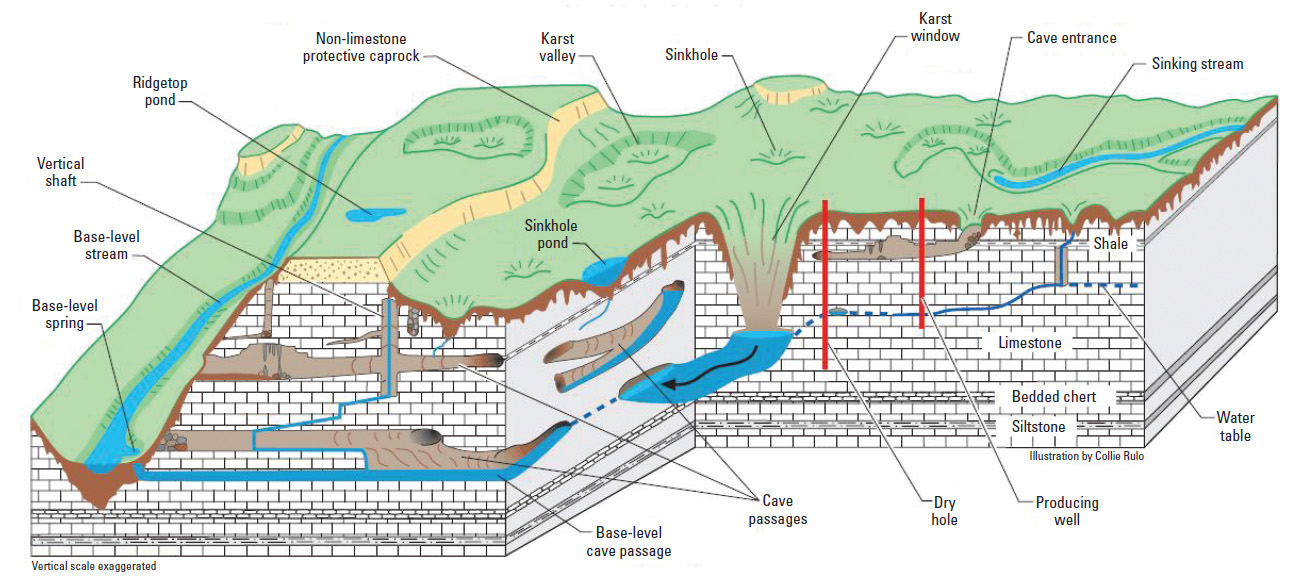
\includegraphics[width=\linewidth]{obrazky/karst/KarstterrainUSGS}
	\caption{Tvary krasového reliéfu (Upraveno podle \textcite{currensGeneralizedBlockDiagram2001})}
	\label{fig:karstterrainusgs}
\end{figure*}

\subsection{Povrchové tvary}
Povrchové tvary se nazývají souhrnně \emph{exokras}. 

\subsubsection{Škrapy}
Nejmenší povrchovým tvarem jsou \emph{škrapy} (\textit{karren)}. Jedná se o malé zařezy či rýhy a jiné vyhloubeniny. Pokud škrapy pokrývají větší plochy, označují se jako \emph{škrapová pole} (\textit{karren field}). \emph{Žlábkové škrapy}  se vyskytují na ukloněných površích. Jedná se o zhruba rovnoběžné žlábky v rovnoměrných rozestupech orientované ve směru spádu. \emph{Stružkové škrapy} jsou drobné rýhy o hloubce \SIrange{1}{2}{\centi\metre}, obdobné šířky a v délce do \SI{0,5}{\metre}. \emph{Puklinové škrapy}  jsou vázané na puklinové systémy, spáry mezi vrstvami apod. Tvar a hustota škrapů je dána charakterem puklinových systémů, jejich hustotou apod. \emph{Mísovité škrapy} se vyskytují na horizontálních površích. Jejich průměr je od několika centimetrů až po metry. Hloubka se pohybuje od pár milimetrů až po cca půl metru. \emph{Šlápovité škrapy} lze také najít na plochých skalních površích. Jedná se o malé stupně široké \SIrange{0,2}{1,0}{\metre} a vysoké několik centimetrů. V půdorysu mají charakter podkovy. \emph{Zaoblené škrapy} vznikají pod vegetací či půdou. Charakterem jsou podobné žlábkovým škrapům.

Větší, \SIrange{2}{4}{\metre} široké a řádově první metry hluboké přímočaré rýhy nazýváme \emph{bogazy}


\begin{figure}[h]
	\centering
	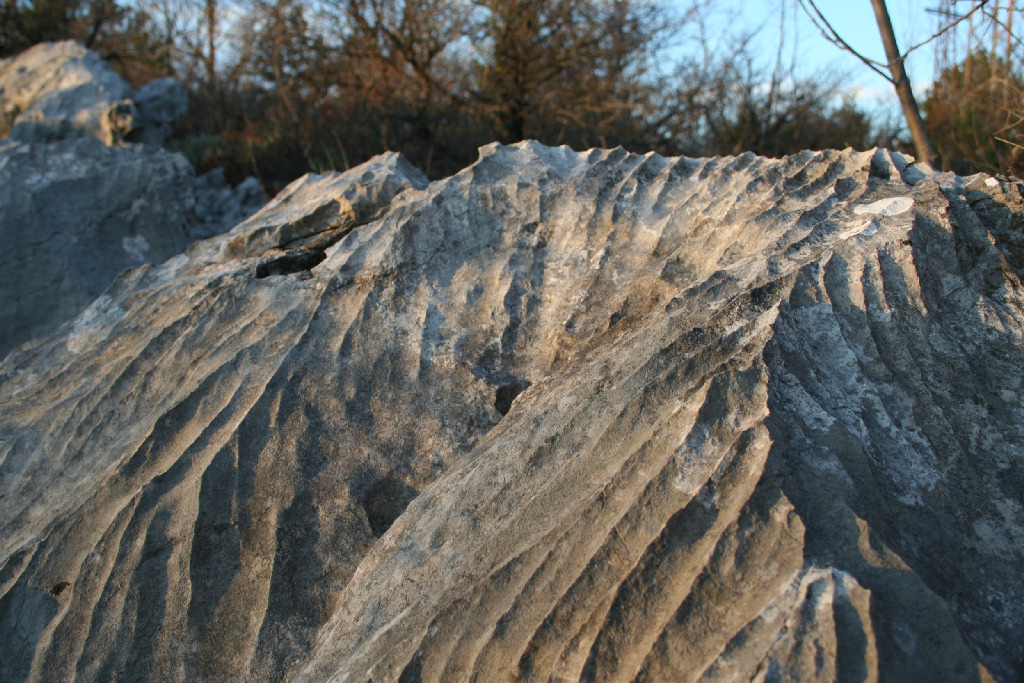
\includegraphics[width=1\linewidth]{obrazky/karst/skrapy1}
	\caption{Ukázka škrapů (Autor: Ekočlen, CC BY-SA 2.5, via Wikimedia Commons)}
	\label{fig:skrapy1}
\end{figure}

\subsubsection{Závrty}
\emph{Závrty} patří již k větším povrchovým útvarům. Jsou to uzavřené deprese rozličných rozměrů. Jejich šířka je zpravidla větší než hloubka. Svou podobou mohou připomínat trychtýř nebo mísy. Průměr závrtů je v řádu metrů až prvních stovek metrů. Na dně závrtů se nachází materiál naplavený vodou mizící v závrtu. Závrty podle způsobu jejich vzniku dělíme na:

\begin{itemize}
	\item disoluční
	\item řícené
	\item sufózní
	\item subsidenční
\end{itemize} 

\emph{Disoluční závrty} vznikají v místech intenzivnějšího rozpouštění (například na křížení dvou puklin). Rozpouštěním se snižuje povrch a vzniká sníženina, která dokáže zachytávat větší a větší množství vody -- dochází tam k pozitivní zpětné vazbě. Vývoj disolučního závrtu ale může být zastaven ucpáním odtoku ze dna závrtu nerozpustným materiálem. \emph{Řícené závrty} vznikají zřícením stropů podzemních prostor. Iniciální stádia mají strmé stěny. Dalším vývoje ale mohou být rozšířené do trychtýřovitého tvaru. Splavováním zvětralinového pokryvu a půdy do podzemí prostřednictvím rozšířených puklin a sufozních kanálů vznikají \emph{sufózní závrty}. Vývoj \emph{subsidenčních závrtů} je spojen s postupným sesedáním nadložních hornin bez jejich znatelného porušení vznikají.

\begin{figure}[h]
	\centering
	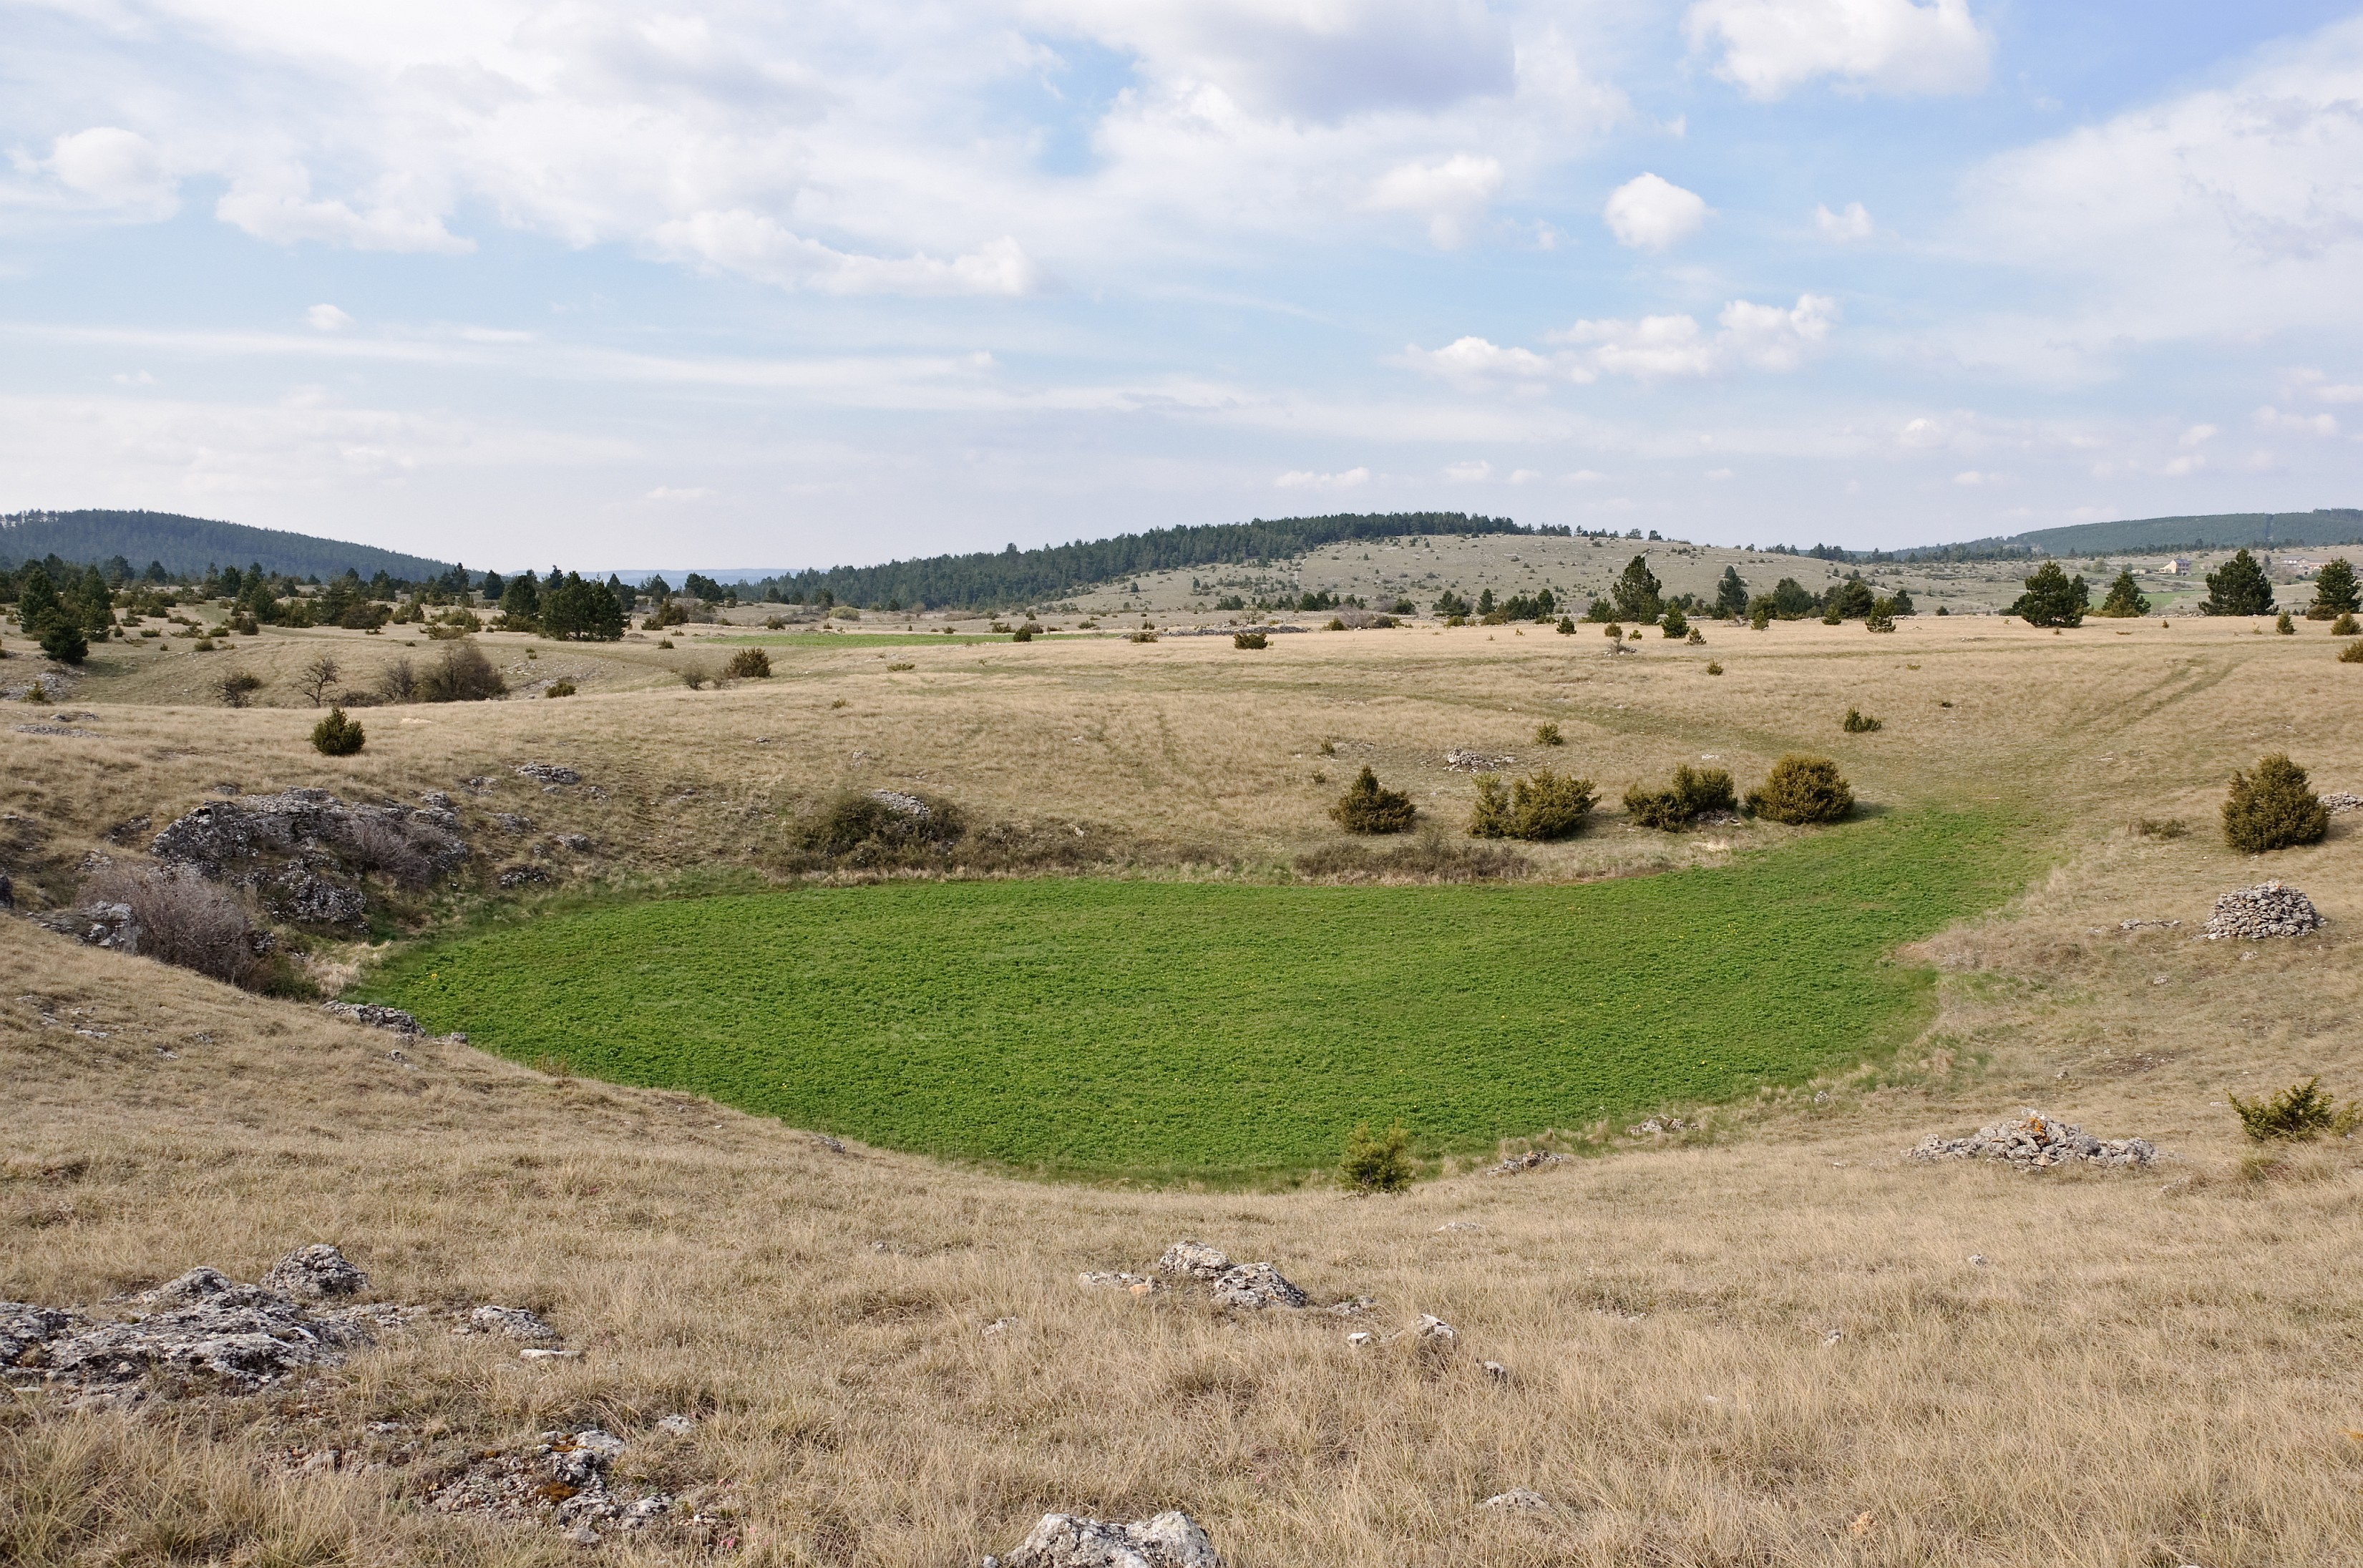
\includegraphics[width=1\linewidth]{obrazky/karst/doline}
	\caption{Závrt v  devez des Cheyrouses, Causse de Sauveterre, Lozère, Francie (Autor: Myrabella, CC BY-SA 3.0, Wikimedia Commons)}
\end{figure}

\emph{Cenoty} jsou specifickou formou závrtů, které jsou vyplněny vodou. Známé jsou cenoty například z poloostrova Yucatán.

\begin{figure}[h]
	\centering
	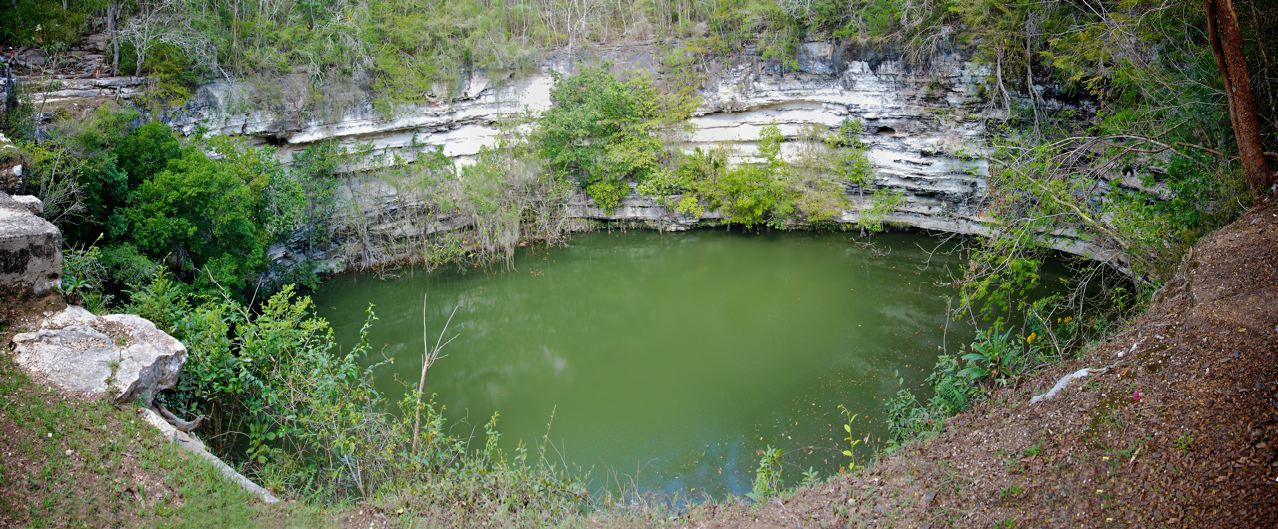
\includegraphics[width=1\linewidth]{obrazky/karst/Mexico_Cenotes}
	\caption{Cenote de los Sacrificios v Chichén Itzá, Yucatánský poloostrov, Mexiko (Autor: Emil Kehnel, CC BY 3.0)}
\end{figure}

\subsubsection{Uvala, polje a krasová údolí}
\emph{Úvala} vznikají spojením závrtů. Bývají protažené pokud sledují průběh šikmě uložených vrstev nebo zlomu. 

Plošně nejrozsáhlejší jsou \emph{polje}. Označujeme tak velké, ze všech stran uzavřené sníženiny, které mají strmé okrajové svahy a ploché dno. Polje nabývá rozměrů větších úval až po stovky \si{\kilo\metre\squared}. Polje mohou být suchá, jiná zas periodicky nebo celoročné vyplněná jezerem. Rozlišujeme tři základní druhy. \emph{Okrajová nebo hraniční polje} jsou ovlivněné řekou, která přitéká z nekrasové oblasti. \emph{Strukturní polje} jsou ovliněné geologickou strukturou.   

\emph{Krasová údolí} mohou mít charakter slepých či poloslepých údolí. \emph{Poloslepá údolí} jsou uzavřená stěnou, za kterou pokračuje suché údolí. Při vyšších vodních stavech může být uzávěrová stěna překonána a suché údolí může být zaplavené. Pokud je stěna, která údolí uzavírá vysoká a údolí za ní nepokračuje, jedná se o \emph{slepé údolí}.

%\emph{Cockpit} je typ krasového reliéfu, který vzniká humidních oblastech. Jedná se o velké množství propojených závrtů, mezi kterými se ční krasové věže a kupy. Může tak připomínat plato na vejce. 

\subsubsection{Tropický kuželový kras}
Teplé a vlhké oblasti jsou příhodné pro rozvoj krasu z důvodu intenzivního chemického zvětrávání. Rychlý rozvoj závrtů vede k destrukci původního povrchu a vzniku tzv. \emph{kuželového krasu} (\textit{cone karst}). Kuželový kras je rozdělován do dvou základních typů: cockpit a věžový kras.

\emph{Cockpit} má charakter zaoblených kopečků a sníženin připomínající v půdorysu mořské hvězdice. Svou podobou může připomínat i plato na vejce. 

\emph{Věžový kras} je typický vysokými věžemi -- \emph{mogoty}. Ty jsou vysoké i přes \SI{100}{\metre} a mají strmé až převislé stěny. 


%TODO Travertiny a pěnovce

\subsection{Podpovrchové tvary}
Nejznámějším podpovrchovým tvarem jsou určitě \emph{jeskyně}. Definic jeskyně je několik. Záleží na úhlu pohledu. Obecně je jeskyně podzemní dutina zcela nebo z velké části omezená matečnou horninou. Podle speleologů musí jeskyně dovolovat vstup a průchod dospělému člověku (i plazením). Z pohledu hydrogeologů musí umožňovat vodě turbulentní pohyb.

\emph{Syngenetické jeskyně} (dutiny) vznikly současně se vznikem horniny (např. lávové jeskyně).  \emph{Epigenetické jeskyně} naopak vznikly až následnými procesy (krasovými, ale i nekrasovými). 

Krasové jeskyně vznikají \emph{korozní a erozní činností kolující vody} v podzemní části krasových oblastí a jejich sekundárním vyplňováním krasovými nebo nekrasovými hmotami.

%TODO: jeskyně
Rozlišujeme tři stádia vývoje jeskyně: iniciální, zralosti a destrukce.

Jeskyně mohou být syngenetické a epigenetické.

Puklinové a vrstevní

Typy jeskyní podle příčného profilu
\emph{Vertikální jeskyně} jsou vázané na svislé tektonické poruchy, kterými vtéká voda do podzemí a postupně je rozšiřuje. Mají mnoho podob a rozměrů: propasti, komíny a podobně.

\emph{Horizontální jeskyně} jsou často spojené s vývojem povrchové údolní sítě. Mají hlavně horizontální nebo subhorizontální charakter: chodby, koridory, haly dómy. 
%Proudící voda v jeskyni působí mechanicky a korozně. Vznikají tak obří hrnce 

%\todo[inline]{vznik jeskyní, proces, obrázky apod}
%Vazba jeskyní na erozní bázi na povrchu – jeskynní úrovně (vznik jeskyní je vázán na polohu erozní báze)
%Jeskynní patro
%
%Eforace, evorze, egutace
\subsubsection{Podpovrchové tvary - sekundární}
Výplň jeskyně může být tvořena materiálem, který byl do ní naplaven zvenčí (\emph{alochtonní} materiál). \emph{Autochtonní} hmoty jsou tvořené resedimentací uhličitanu vápenatého (sintry) Výplň jeskyně nazýváme speleotémy. 

Do stropních speleotémů patří \emph{brčka} (\textit{straw stalaktite}), které jsou základním tvarem stalaktitu, samotné \emph{stalaktity}, ale i další formy jako např. záclony a závěsy. Z kapek vody, která dopadá na podlahu vznikají podlahové speleotémy. Rostou směrem vzhůru. Zde patří \emph{stalagmity}. Spojením proti sobě rostoucího stalaktitu a stalagmitu vzniká \emph{stalagnát}. Na podlahách jeskyň ale můžeme najít i další tvary jako např sintrové hráze, sintrové náteky, sintrové kupy či gejzírové stalagmity. Stěny jeskyň jsou pokryté různými sintrovými povlaky, vodopády, výkvěty, štíty. Mezi volné sintrové tvary se řadí jeskynní perly, vápencové škraloupy.


\newpage
\onecolumn
\begin{boxotazky}{Kontrolní a klíčové otázky, na které bychom měli znát odpověď}
	\begin{itemize}
		\item 
		\item 
		
	\end{itemize}
\end{boxotazky}

\begin{boxslovnik}{Další klíčové pojmy k zapamatování}
	aaa & adfasd \\
	
\end{boxslovnik}
\twocolumn